% Configurazione
\documentclass[12pt, a4paper]{report}

\usepackage{graphicx}
\usepackage[table,xcdraw]{xcolor}
%\usepackage{xcolor}
\usepackage{float}
\usepackage{titlesec}
\usepackage[utf8]{inputenc}
\usepackage{hyperref}
\hypersetup{
    colorlinks=true,
    linkcolor=black,
    urlcolor=blue,
    }
\graphicspath{ {immagini/} }
\definecolor{RossoUnipd}{HTML}{B5121B}
\titleformat{\chapter}{\normalfont\huge}{\thechapter.}{20pt}{\huge\textbf}
\renewcommand{\contentsname}{Indice}
\newcommand{\todo}[1]{\textcolor{red}{TODO: #1}}

% Variabili
\newcommand{\titolo}{Analisi dei Requisiti}



% Struttura
\begin{document}
  \begin{minipage}[]{0.3\textwidth}
  
\includegraphics[width=0.7\textwidth]{logo_uni}
\end{minipage}
\begin{minipage}[]{0.6\textwidth}
  \textcolor{RossoUnipd}{
    \textbf{Università degli Studi di Padova} \\
    Laurea: Informatica \\
    Corso: Ingegneria del Software \\
    Anno Accademico: 2021/2022
  }
\end{minipage}

\bigskip

\begin{minipage}[]{0.3\textwidth}
  
\includegraphics[width=0.7\textwidth]{logo_merl}
\end{minipage}
\begin{minipage}[]{0.6\textwidth}
  Gruppo: MERL \\
  Email: \texttt{merlunipd@gmail.com}
\end{minipage}

\bigskip
\bigskip
\bigskip

  \begin{center}
  \Huge\textbf{\titolo}
\end{center}

\bigskip
\bigskip
\bigskip
  \newpage
  \begin{center}
  \huge{Registro delle Modifiche}
\end{center}
\newcommand{\aCapo}[1]{%
  \begin{tabular}{@{}c@{}}\strut#1\strut\end{tabular}%
}
\begin{center}
  \begin{tabular}{|p{2cm}|p{2cm}|p{4cm}|p{5cm}|}
    \hline
    \textbf{Versione} & \textbf{Data} & \textbf{Autore/Verificatore} & \textbf{Modifica}                    \\ \hline
    v0.1.4            & 15/01/2022    & \aCapo{Marco Mamprin\\Mattia Zanellato} & Aggiunte sottosezione "Testing"  \\ \hline  
    v0.1.3            & 09/01/2022    & \aCapo{Marco Mamprin\\Emanuele Pase} & Aggiunte sottosezione "Metriche"  \\ \hline           
    v0.1.2            & 07/01/2022    & \aCapo{Riccardo Contin\\Marko Vukovic} & Aggiunte sottosezioni "Preventivo" e "Consuntivo"  \\ \hline
    v0.1.1            & 02/01/2022    & \aCapo{Marko Vukovic\\Emanuele Pase} & Aggiunta sezione automazione  \\ \hline
    v0.1.0            & 27/12/2021    & Riccardo Contin & Approvazione  \\ \hline
    v0.0.13           & 24/12/2021    & \aCapo{Emanuele Pase\\Marco Mamprin} & Fix minori  \\ \hline
    v0.0.12           & 24/12/2021    & \aCapo{Lorenzo Onelia\\Emanuele Pase} & Fix minori \\ \hline
    v0.0.11           & 21/12/2021    & \aCapo{Marko Vukovic\\Marco Mazzucato} & Aggiunta sezione "Gestione dei Processi Organizzativi" \\ \hline
    v0.0.10            & 18/12/2021    & \aCapo{Emanuele Pase\\Marco Mazzucato} & Aggiunta sezione "Sviluppo" \\ \hline
    v0.0.9            & 17/12/2021    & \aCapo{Mattia Zanellato\\Lorenzo Onelia} & Aggiunta sezione "Fornitura" \\ \hline
    v0.0.8            & 17/12/2021    & \aCapo{Mattia Zanellato\\Lorenzo Onelia} & Aggiunto capitolo "Introduzione" \\ \hline
    v0.0.7            & 16/12/2021    & \aCapo{Marco Mazzucato\\Marco Mamprin} & Aggiunta sezione "Documentazione" \\ \hline
    v0.0.6            & 14/12/2021    & \aCapo{Marco Mamprin\\Riccardo Contin} & Aggiunta sezione "Formazione" \\ \hline
    v0.0.5            & 14/12/2021    & \aCapo{Marco Mamprin\\Riccardo Contin}   & Aggiunta sezione "Validazione" \\ \hline
    v0.0.4            & 14/12/2021    & \aCapo{Marco Mamprin\\Riccardo Contin}   & Aggiunta sezione "Gestione della Qualità" \\ \hline
    v0.0.3            & 11/12/2021    & \aCapo{Lorenzo Onelia\\Emanuele Pase} & Aggiunta sezione "Verifica" \\ \hline
    v0.0.2            & 10/12/2021    & \aCapo{Emanuele Pase\\Riccardo Contin}  & Aggiunta sezione "Gestione della configurazione" \\ \hline
    v0.0.1            & 08/12/2021    & \aCapo{Marko Vukovic\\Marco Mazzucato}   & Aggiunta sezione "Infrastruttura" \\ \hline
    v0.0.0            & 07/12/2021    & \aCapo{Marko Vukovic\\Marco Mazzucato}   & Creata prima struttura del documento \\ \hline
  \end{tabular}
\end{center}

  \tableofcontents

  % Capitoli
  \chapter{Introduzione}

\section{Scopo del documento}

Il \textit{Piano di Progetto} è un documento di fondamentale importanza per riuscire a lavorare nel migliore dei
modi. La sua struttura è:
\begin{itemize}
    \item \textbf{Analisi dei rischi: } permette di indicare i possibili rischi, la probabilità che essi si verifichino e la loro gravità;
    \item \textbf{Pianificazione: } permette di pianificare le milestone;
    \item \textbf{Preventivo: } permette di indicare le ore e i costi che si intende impiegare in ogni periodo pianificato;
    \item \textbf{Consuntivo: } permette di analizzare il reale svolgimento dei periodi passati rispetto a com'erano stati preventivati;
    \item \textbf{Mitigazione dei rischi: } permette di analizzare i rischi che si sono effettivamente verificati. 
\end{itemize}

\section{Glossario}

Nel caso ci fossero termini che provocano difficoltà di interpretazione o che risultano ambigui, esiste un \textit{Glossario}
che contiene una serie di termini con relativa descrizione che fornisce un supporto alla consultazione del documento.

\section{Riferimenti}
\subsection{Riferimenti normativi}
\begin{itemize}
  \item \textit{Norme di Progetto}
  \item Capitolato d'appalto C5 - Zucchetti S.p.A.: Login Warrior \\
  \url{https://www.math.unipd.it/~tullio/IS-1/2021/Progetto/C5.pdf}
\end{itemize}

\subsection{Riferimenti informativi}
\begin{itemize}
  \item Slide T5 - Corso di Ingegneria del Software - Il ciclo di vita del SW \\
  \url{https://www.math.unipd.it/~tullio/IS-1/2021/Dispense/T05.pdf}
  \item Slide T6 - Corso di Ingegneria del Software - Gestione di progetto \\
  \url{https://www.math.unipd.it/~tullio/IS-1/2021/Dispense/T06.pdf}
\end{itemize}

  \chapter{Descrizione}

\section{Obiettivi del Prodotto}
Il prodotto deve essere in grado di visualizzare dati a molte dimensioni sotto forma di diversi grafici, per supportare la fase di analisi attraverso l'utilizzo di tecnologie web.

\section{Funzioni del Prodotto}
L'applicazione si occupa di analizzare uno o più set di dati e di restituire dei grafici che risultano essere più comprensibili e significativi.
Con l'utilizzo di grafici appositamente creati e in base a filtri selezionati dall'utente che permettono varie visualizzazioni, è possibile estrapolare informazioni che in un primo momento potevano essere poco chiare o nascoste.
È possibile anche salvare le informazioni in un file scaricabile in formato JSON, in modo da poter successivamente ripristinare la sessione nel punto in cui era stata interrotta.

\section{Vincolo}
\todo{Da discutere e quindi poi implementare}

  \chapter{Casi d'Uso}

\todo{rivedere la numerazione dei casi d'uso}

\begin{figure}[h]
  \centering
  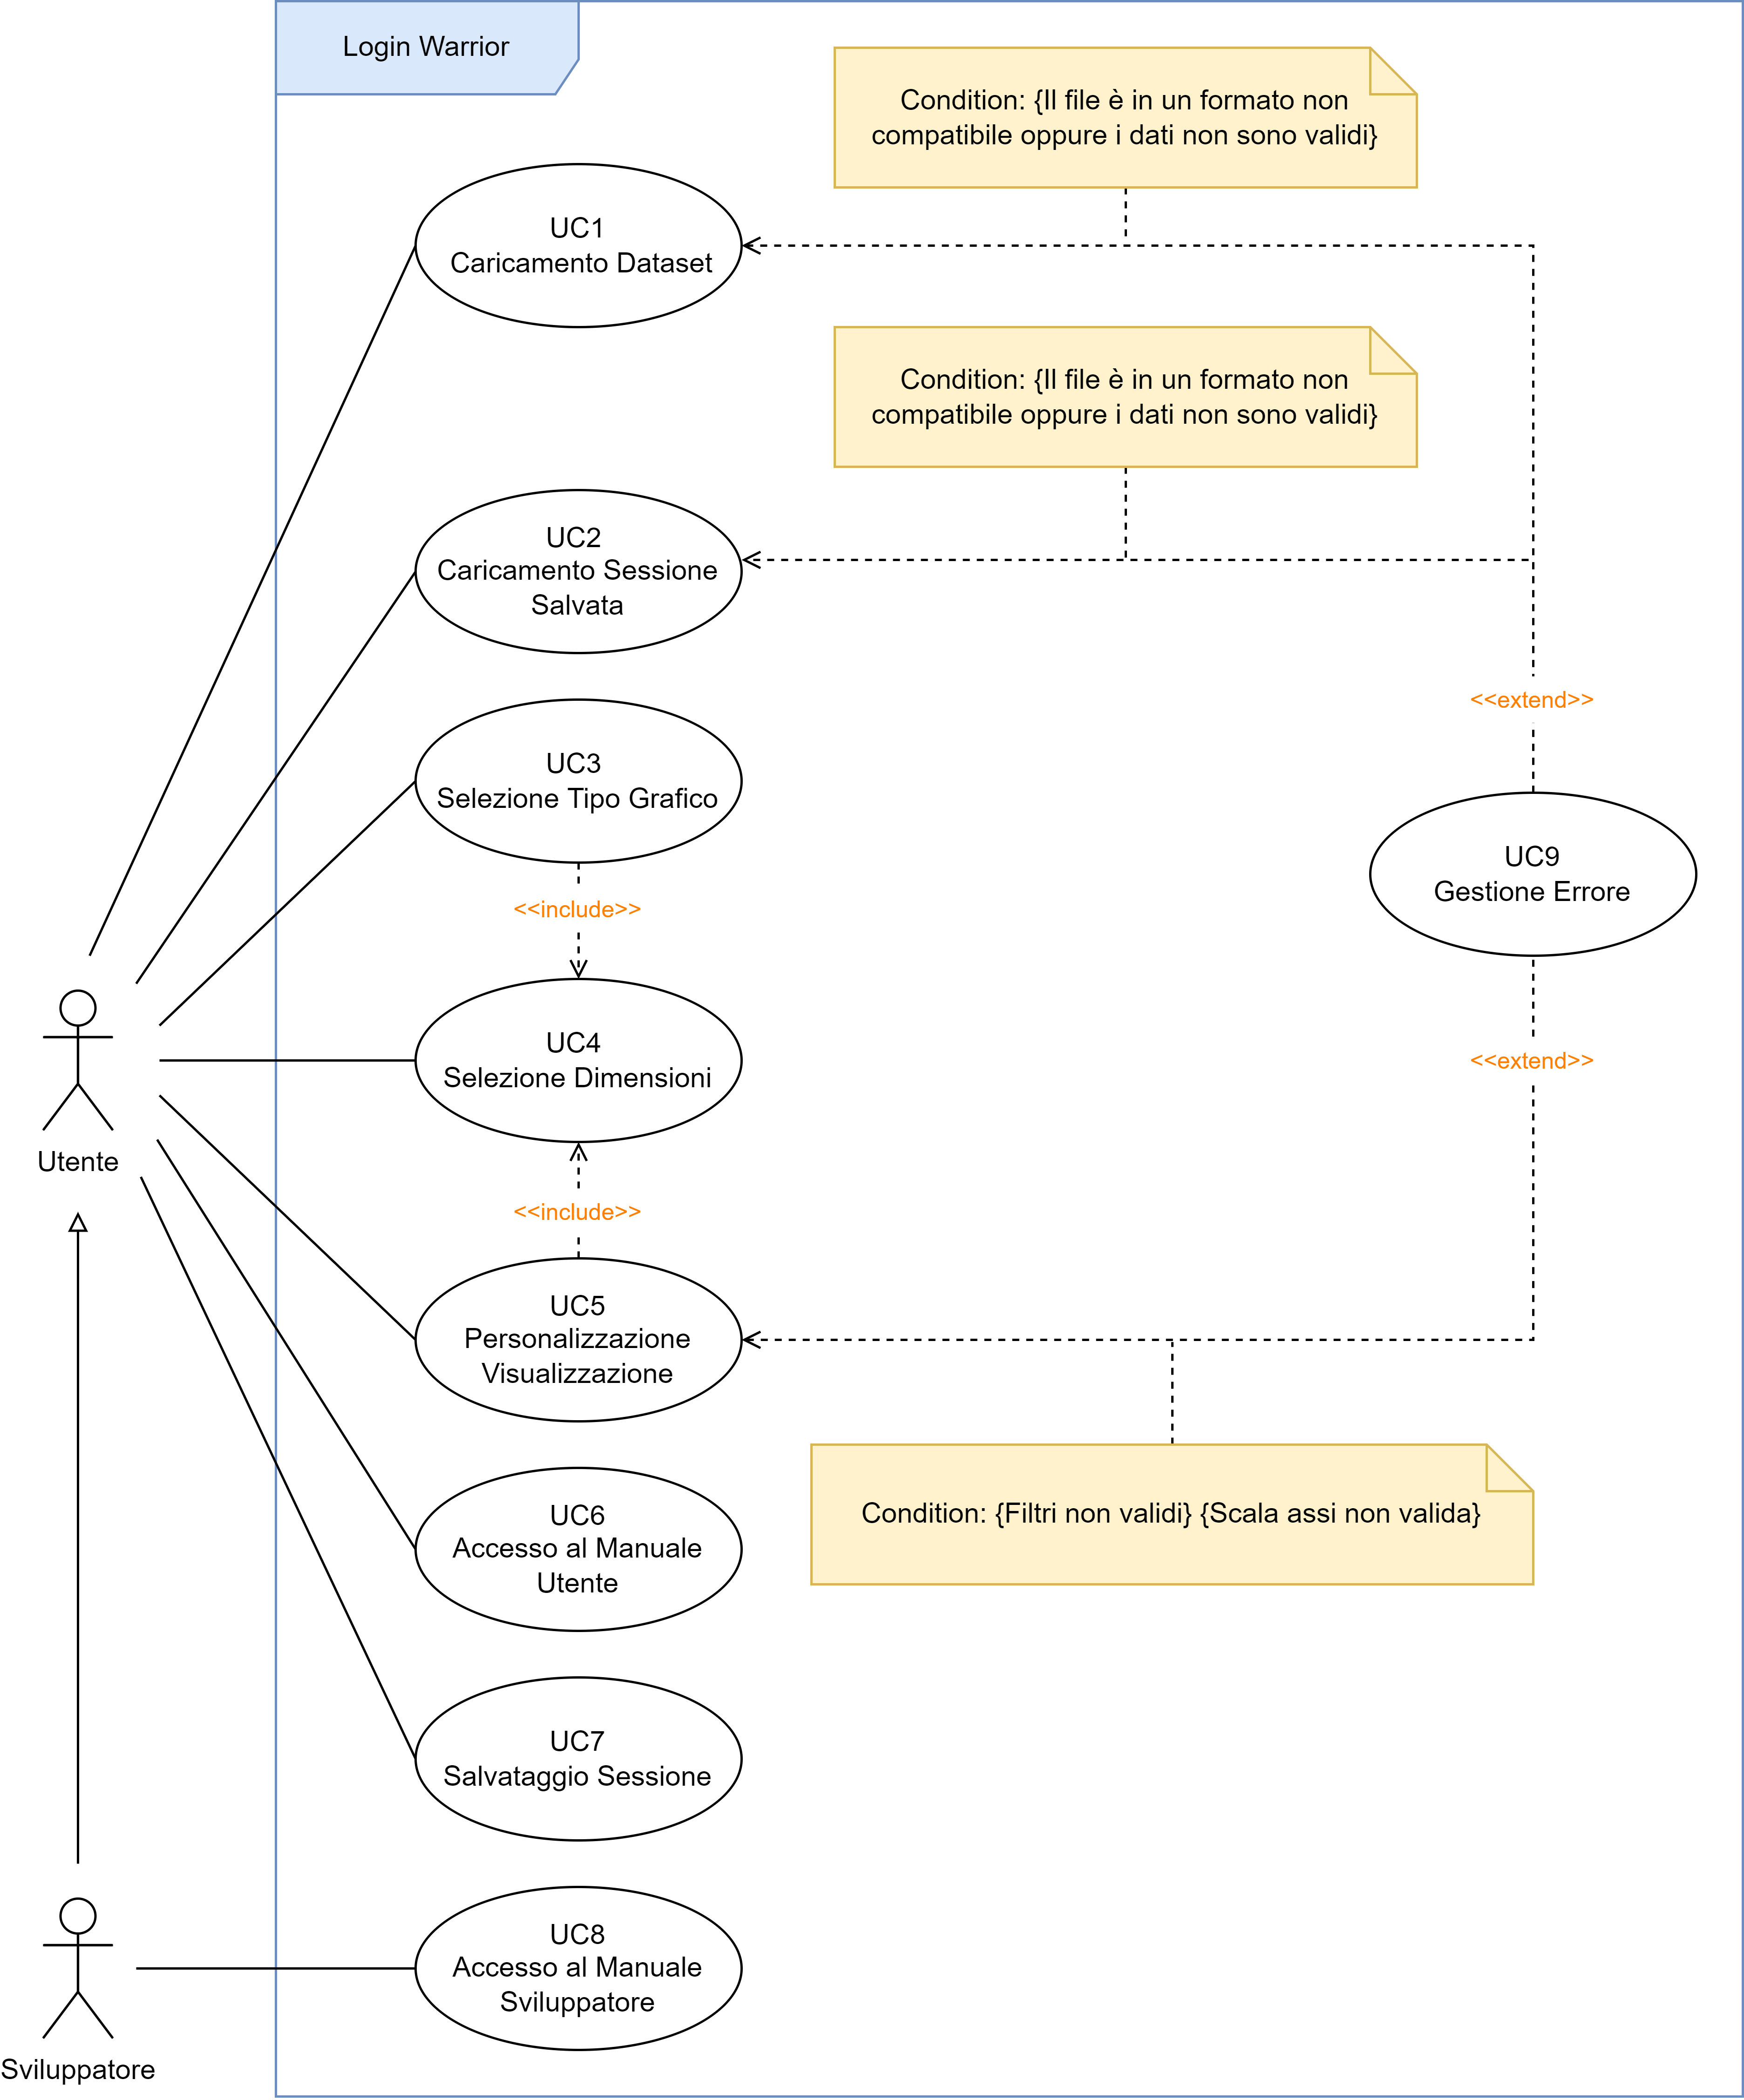
\includegraphics[width=0.6\textwidth]{UML_general}
  \caption{Inizializzazione del sistema}
\end{figure}
\section{UC1 - Caricamento dataset}
\begin{itemize}
  \item \textbf{Descrizione:} l'utente vuole analizzare un nuovo dataset non presente nel sistema;
  \item \textbf{Attore primario:} utente;
  \item \textbf{Precondizioni:} il sistema è raggiungibile e funzionante. L’utente ha a disposizione un dataset in formato CSV;
  \item \textbf{Postcondizioni:} i dati presenti nel file vengono caricati nel sistema. Viene visualizzato un messaggio che indica il corretto caricamento dei dati;
  \item \textbf{Scenario principale:}
  \begin{enumerate}
    \item L'utente accede al sistema;
    \item L'utente sceglie un file in formato CSV presente in locale e lo carica nel sistema;
    \item L'utente è pronto ad analizzare i dati.
  \end{enumerate}
  \item \textbf{Estensioni:} nel caso in cui il file sia in un formato non valido o i dati non siano validi:
    \begin{enumerate}
      \item Il caricamento non va a buon fine;
      \item Viene visualizzato un errore esplicativo [UC9].
    \end{enumerate}
\end{itemize}

\section{UC2 - Caricamento sessione salvata}
\begin{itemize}
  \item \textbf{Descrizione:} l'utente vuole riprendere ad analizzare da dove si era interrotto
  o ha la necessità di visualizzare una sessione precedente;
  \item \textbf{Attore Primario:} utente;
  \item \textbf{Precondizioni:} l'utente che avvia l'applicativo ha salvato almeno una sessione di lavoro precedente;
  \item \textbf{Postcondizioni:} i dati di una sessione precedentemente salvata vengono ricaricati nel sistema. Viene visualizzato un messaggio che indica il corretto caricamento dei dati;
  \item \textbf{Scenario Principale:}
  \begin{enumerate}
    \item L'utente accede al sistema;
    \item L'utente sceglie la sessione da caricare selezionando il file JSON desiderato tra quelli disponibili,
    cioè tra le sessioni salvate in precedenza;
    \item L'utente riprende da dove aveva salvato.
  \end{enumerate}
  \item \textbf{Estensioni:} nel caso in cui il file JSON selezionato non è leggibile per qualche possibile errore di salvataggio:
    \begin{enumerate}
      \item Fallisce il caricamento della sessione precedente;
      \item Viene visualizzato un errore esplicativo [UC9].
    \end{enumerate}
\end{itemize}


\section{UC3 - Selezione dimensioni}
 \begin{itemize}
     \item \textbf{Descrizione:} selezione dimensioni con cui verrà visualizzato il grafico;
     \item \textbf{Attore primario:} utente;
     \item \textbf{Precondizioni:} il sistema è stato inizializzato [UC1];
     \item \textbf{Postcondizioni:} le dimensioni vengono aggiornate nel sistema;
     \item \textbf{Scenario principale:}
     \begin{enumerate}
         \item vengono mostrate all'utente le dimensioni di default e altre dimensioni tra cui scegliere;
         \item l'utente seleziona la/e dimensione/i che più ritiene utile/i.
     \end{enumerate}
 \end{itemize}


\section{UC4 - Selezione tipo di grafico}
\begin{figure}[H]
 \includegraphics[width=\textwidth]{uc4.png}
 \vspace{-5mm}
 \caption*{Figura 2: UC4 - Selezione tipo di grafico}
\end{figure}

 \begin{itemize}
     \item \textbf{Descrizione:} viene visualizzata la scelta della tipologia di grafico;
     \item \textbf{Attore primario:} utente;
     \item \textbf{Precondizioni:} il sistema è stato inizializzato [UC1];
     \item \textbf{Postcondizioni:} viene visualizzato il grafico desiderato;
     \item \textbf{Scenario principale:} l'utente sceglie la visualizzazione più consona tra quelle disponibili;
     \item \textbf{Generalizzazioni:} l'utente può selezionare una tra le possibili opzioni:
     \begin{enumerate}
         \item \textit{Scatter Plot} [UC4.1];
         \item \textit{Parallel Coordinates} [UC4.2];
         \item \textit{Force Directed Graph} [UC4.3];
         \item \textit{Diagramma di Sankey} [UC4.4].
     \end{enumerate}
 \end{itemize}


\section{UC4 - Personalizzazione Visualizzazione}

\begin{figure}[h]
  \centering
  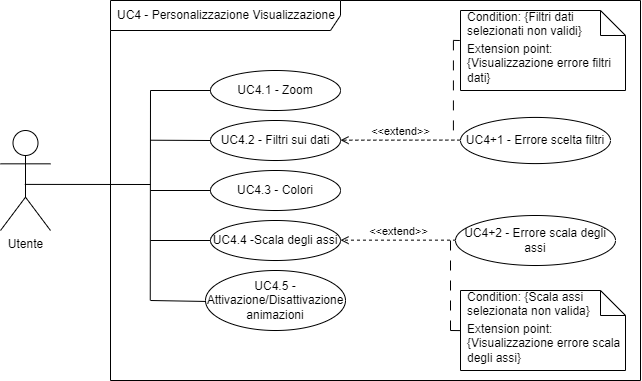
\includegraphics[width=0.6\textwidth]{ucX.png}
  \caption{UC4 - Personalizzazione Visualizzazione}
\end{figure}

\begin{itemize}
  \item \textbf{Descrizione}: l'utente ha la possibilità di modificare vari aspetti visivi del grafico;
  \item \textbf{Attore primario}: utente;
  \item \textbf{Precondizioni}: l'utente ha selezionato le dimensioni del grafico [UC3] e l'applicativo lo ha generato;
  \item \textbf{Postcondizioni}: le modifiche apportate al grafico vengono visualizzate;
  \item \textbf{Scenario principale}:
  \begin{itemize}
    \item L'utente può scegliere le caratteristiche da modificare tra:
      \begin{itemize}
        \item Zoom [UC4.1];
        \item Filtri sui dati [UC4.2];
        \item Colori [UC4.3];
        \item Scala degli assi [UC4.4];
        \item Attivare/Disattivare le animazioni [UC4.5];
      \end{itemize}
    \item Il grafico viene visualizzato con le nuove caratteristiche;
  \end{itemize}
  \item \textbf{Estensioni}:
    \begin{itemize}
      \item L'utente inserisce dei filtri non validi [UC 4 + 1];
      \item L'utente inserisce una scala degli assi non valida [UC4 + 2].
    \end{itemize}
\end{itemize}

\section{UC4 + 1 - Errore scelta filtri}
\begin{itemize}
  \item \textbf{Descrizione}: l'utente sceglie dei filtri non validi;
  \item \textbf{Attore primario}: utente;
  \item \textbf{Precondizioni}: l'utente sceglie dei filtri che non permettono una corretta visualizzazione del grafico;
  \item \textbf{Postcondizioni}: l'utente visualizza un messaggio di errore;
  \item \textbf{Scenario principale}:
    \begin{itemize}
      \item L'utente visualizza un messaggio di errore esplicativo;
      \item L'utente clicca \texttt{Capito} per tornare alla visualizzazione del grafico con la personalizzazione di default.
    \end{itemize}
\end{itemize}

\section{UC4 + 2 - Errore scala degli assi}
\begin{itemize}
  \item \textbf{Descrizione}: l'utente scelglie una scala non valida;
  \item \textbf{Attore primario}: utente;
  \item \textbf{Precondizioni}: l'utente sceglie una scala degli assi che non permette una corretta visualizzazione del grafico;
  \item \textbf{Postcondizioni}: l'utente visualizza un messaggio di errore;
  \item \textbf{Scenario principale}:
    \begin{itemize}
      \item L'utente visualizza un messaggio di errore esplicativo;
      \item L'utente clicca \texttt{Capito} per tornare alla visualizzazione del grafico con la personalizzazione di default.
    \end{itemize}
\end{itemize}

\section{Accesso ai manuali}
\begin{figure}[h]
  \centering
  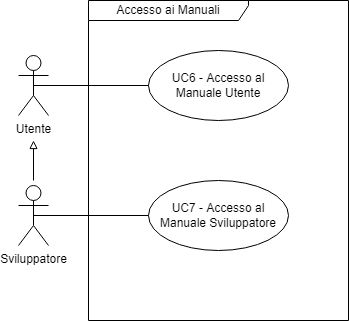
\includegraphics[width=0.6\textwidth]{UC_manuali}
  \caption{UC6 UC7 - Accesso ai manuali utente e sviluppatore}
\end{figure}
\subsection{UC6 - Accesso al Manuale Utente}

\begin{itemize}
  \item \textbf{Descrizione}: l'utente che ha un dubbio o vuole più informazioni sull'utilizzo dell'applicazione, deve avere accesso rapido al manuale utente;
  \item \textbf{Attore primario}: utente;
  \item \textbf{Precondizioni}: nessuna, l'opzione di accesso ai manuali deve essere sempre disponibile all'utente;
  \item \textbf{Postcondizioni}: viene visualizzato il manuale utente;
  \item \textbf{Scenario principale}:
  \begin{enumerate}
    \item L'utente seleziona il "manuale utente";
    \item Viene visualizzato il manuale utente.
  \end{enumerate}
\end{itemize}

\subsection{UC7 - Accesso al Manuale Sviluppatore}

\begin{itemize}
  \item \textbf{Descrizione}: essendo Login Warrior un progetto open source, un qualsiasi sviluppatore deve avere accesso ad un manuale sviluppatore (sia per manutenzione, sia per estendere il software);
  \item \textbf{Attore primario}: sviluppatore;
  \item \textbf{Precondizioni}: nessuna, l'opzione di accesso ai manuali deve essere sempre disponibile allo sviluppatore;
  \item \textbf{Postcondizioni}: viene visualizzato il manuale sviluppatore;
  \item \textbf{Scenario principale}:
  \begin{enumerate}
    \item Lo sviluppatore seleziona il "manuale sviluppatore";
    \item Viene visualizzato il manuale sviluppatore.
  \end{enumerate}
\end{itemize}

\section{UC6 - Salvataggio Sessione}

\begin{itemize}
  \item \textbf{Descrizione:} l'utente salva la sessione di lavoro;
  \item \textbf{Attore primario:} utente;
  \item \textbf{Precondizioni:} l'utente ha svolto una sessione di lavoro sull'applicazione, in particolare potrebbe aver scelto un grafico specifico, impostato le dimensioni volute e modificato i parametri personalizzando la visualizzazione;
  \item \textbf{Postcondizioni:} l'utente possiede un file JSON in grado di recuperare grafico, dimensioni e parametri impostati durante la sessione di lavoro;
  \item \textbf{Scenario principale:}
  \begin{enumerate}
    \item L'utente sta lavorando sull'applicazione;
    \item L'utente seleziona la funzionalità ``Salvataggio Sessione'';
    \item L'utente seleziona la directory in cui salvare il file JSON.
  \end{enumerate}
\end{itemize}

\section{UC9- Gestione errore}
\begin{itemize}
  \item \textbf{Attore Primario:} utente;
  \item \textbf{Precondizioni:} l'utente compie un'azione che fa fallire il corretto funzionamento dell'applicazione;
  \item \textbf{Postcondizioni:} l'utente visualizza un messaggio di errore e l'azione non va a buon fine.
  \item \textbf{Scenario Principale:}
  \begin{enumerate}
    \item L'utente visualizza un messaggio di errore esplicativo;
  \end{enumerate}
\end{itemize}

  \chapter{Requisiti}

\section{Introduzione}
\section{Requisiti Funzionali}
\begin{table}[H]
  \centering
  \begin{tabular}{|c|c|c|c|}
    \hline
    \rowcolor[HTML]{036400}
    {\color[HTML]{FFFFFF} \textbf{Codice}} & {\color[HTML]{FFFFFF} \textbf{Classificazione}} & {\color[HTML]{FFFFFF} \textbf{Descrizione}} & {\color[HTML]{FFFFFF} \textbf{Fonti}} \\ \hline
    \rowcolor[HTML]{EFEFEF}
    &  &  &  \\ \hline
    \rowcolor[HTML]{C0C0C0}
    &  &  &  \\ \hline
  \end{tabular}
  \caption{Tabella dei requisiti funzionali}
\end{table}

\section{Requisiti di Qualità}
\begin{table}[H]
  \centering
  \begin{tabular}{|c|c|c|c|}
    \hline
    \rowcolor[HTML]{036400}
    {\color[HTML]{FFFFFF} \textbf{Codice}} & {\color[HTML]{FFFFFF} \textbf{Classificazione}} & {\color[HTML]{FFFFFF} \textbf{Descrizione}} & {\color[HTML]{FFFFFF} \textbf{Fonti}} \\ \hline
    \rowcolor[HTML]{EFEFEF}
    &  &  &  \\ \hline
    \rowcolor[HTML]{C0C0C0}
    &  &  &  \\ \hline
  \end{tabular}
  \caption{Tabella dei requisiti di qualità}
\end{table}

\section{Requisiti di Vincolo}
\begin{table}[H]
  \centering
  \begin{tabular}{|c|c|c|c|}
    \hline
    \rowcolor[HTML]{036400}
    {\color[HTML]{FFFFFF} \textbf{Codice}} & {\color[HTML]{FFFFFF} \textbf{Classificazione}} & {\color[HTML]{FFFFFF} \textbf{Descrizione}} & {\color[HTML]{FFFFFF} \textbf{Fonti}} \\ \hline
    \rowcolor[HTML]{EFEFEF}
    &  &  &  \\ \hline
    \rowcolor[HTML]{C0C0C0}
    &  &  &  \\ \hline
  \end{tabular}
  \caption{Tabella dei requisiti di vincolo}
\end{table}

\section{Requisiti Prestazionali}
\begin{table}[H]
  \centering
  \begin{tabular}{|c|c|c|c|}
    \hline
    \rowcolor[HTML]{036400}
    {\color[HTML]{FFFFFF} \textbf{Codice}} & {\color[HTML]{FFFFFF} \textbf{Classificazione}} & {\color[HTML]{FFFFFF} \textbf{Descrizione}} & {\color[HTML]{FFFFFF} \textbf{Fonti}} \\ \hline
    \rowcolor[HTML]{EFEFEF}
    &  &  &  \\ \hline
    \rowcolor[HTML]{C0C0C0}
    &  &  &  \\ \hline
  \end{tabular}
  \caption{Tabella dei requisiti prestazionali}
\end{table}

\section{Tracciamento}

\subsection{Fonte - Requisiti}
\begin{table}[H]
  \centering
  \begin{tabular}{|c|c|}
    \hline
    \rowcolor[HTML]{036400}
    {\color[HTML]{FFFFFF} Fonte} & {\color[HTML]{FFFFFF} Requisiti} \\ \hline
    \rowcolor[HTML]{EFEFEF}
    &  \\ \hline
    \rowcolor[HTML]{C0C0C0}
    &  \\ \hline
  \end{tabular}
  \caption{Tabella di tracciamento fonte-requisiti}
\end{table}

\subsection{Requisito - Fonti}
\begin{table}[H]
  \centering
  \begin{tabular}{|c|c|}
    \hline
    \rowcolor[HTML]{036400}
    {\color[HTML]{FFFFFF} Fonte} & {\color[HTML]{FFFFFF} Requisiti} \\ \hline
    \rowcolor[HTML]{EFEFEF}
    &  \\ \hline
    \rowcolor[HTML]{C0C0C0}
    &  \\ \hline
  \end{tabular}
  \caption{Tabella di tracciamento requisito-fonti}
\end{table}

\section{Conclusioni}

\end{document}
